%                                                                 aa.dem
% AA vers. 9.1, LaTeX class for Astronomy & Astrophysics
% demonstration file
%                                                       (c) EDP Sciences
%-----------------------------------------------------------------------
%
%\documentclass[referee]{aa} % for a referee version
%\documentclass[onecolumn]{aa} % for a paper on 1 column  
%\documentclass[longauth]{aa} % for the long lists of affiliations 
%\documentclass[letter]{aa} % for the letters 
%\documentclass[bibyear]{aa} % if the references are not structured 
%                              according to the author-year natbib style

%
% \documentclass[draft]{aa} 
\documentclass{aa}

%
\usepackage{graphicx}
%%%%%%%%%%%%%%%%%%%%%%%%%%%%%%%%%%%%%%%%
\usepackage{txfonts}
%%%%%%%%%%%%%%%%%%%%%%%%%%%%%%%%%%%%%%%%
%\usepackage[options]{hyperref}
% To add links in your PDF file, use the package "hyperref"
% with options according to your LaTeX or PDFLaTeX drivers.
%
\usepackage[]{hyperref}
\hypersetup{colorlinks=true, urlcolor=blue, citecolor=cyan, pdfborder={0 0 0}}

\begin{document} 


\title{A detailed analysis of the most distant catalogued open clusters}
\subtitle{Re-assessing fundamental parameters with Gaia EDR3 and \texttt{ASteCA}}

\author{G. I. Perren\inst{1}
      \and
      M. S. Pera\inst{1}
      \and
      H. Navone\inst{2}
      \and
      R. A. Vázquez\inst{3}
      % \fnmsep\thanks{Just to show the usage
      % of the elements in the author field}
}

\institute{Instituto de Astrof\'isica de La Plata (IALP-CONICET), La Plata,
Argentina\\
\email{gabrielperren@gmail.com}
\and
Facultad de Ciencias Exactas, Ingeniería y Agrimensura (UNR-IFIR-CONICET),
Rosario, Argentina
\and
Facultad de Ciencias Astronómicas y Geofísicas (UNLP-IALP-CONICET), 1900 La
Plata, Argentina
% \thanks{The university of heaven temporarily does not
%         accept e-mails}
}
\date{Received September 15, 2021; accepted December 16, 2021}

% \abstract{}{}{}{}{} 
% 5 {} token are mandatory
 
\abstract
% context heading (optional)
% {} leave it empty if necessary  
{Several studies have been presented in the last few years applying some kind of
automatic processing of data to estimate the fundamental parameters of open
clusters. These parameters are later on employed in larger scale analyses, for
example the structure of the Galaxy's spiral arms.
The distance is one of the more straightforward parameters to estimate, yet
enormous differences can still be found among published data. This is
particularly true for open clusters located more than a few Kpc away.}
% aims heading (mandatory)
{
We cross-matched several published catalogues and selected the twenty-five most
distant open clusters ($>$9000 Kpc). We then performed a detailed analysis of
their fundamental parameters, with emphasis on their distances, to determine the
agreement between catalogues and our estimates.}
% methods heading (mandatory)
{Photometric and astrometric data from the Gaia EDR3 survey was employed. The
data was processed with our own membership analysis code (pyUPMASK), and our
package for automatic fundamental cluster's parameters estimation
(\texttt{ASteCA}).}
% results heading (mandatory)
{We find differences in the estimated distances of up to several Kpc
between our results and those catalogued, even for the catalogues that show the
best matches with \texttt{ASteCA} values. Large differences are also found for
the age estimates.}
% conclusions heading (optional), leave it empty if necessary 
{Caution is thus strongly recommended when using catalogued parameters of open
clusters to infer large-scale properties of the Galaxy, particularly for those
located more than a few Kpc away.}

\keywords{
  Methods: statistical --
  Galaxies: star clusters: general --
  (Galaxy:) open clusters and associations: general --
  Techniques: photometric--
  Parallaxes --
  Proper motions
}

\maketitle


\section{Introduction}

 Open clusters (OCs) are not only used as laboratories to investigate stellar
 evolution, they are also routinely employed in the analysis of the Milky Way's
 structure~\citep{Loktin_1992,Moitinho_2006,Vazquez2008,Moitinho_2010}.
 Young OCs for example are known to be particularly
 useful in the tracing of spiral arms, as they have not yet drifted too far
 from their birth position~\citep{carraro_2013,Molina_2018}. As deeper, more
 complete, and more precise photometric and astrometric data becomes available,
 these studies will inevitably be extended towards more distant regions of the
 Galaxy.

 xxxxx

 This article is structured as follows. In Sect~\ref{sec:cat_clust_data} we
 introduce the stellar cluster catalogues, the clusters selected to be
 analyzed (crossed-matched from those catalogues), and the photometric and 
 astrometric data used to perform the analysis. Sect~\ref{sec:dclust_analy}
 presents the methods employed in the study of all the clusters. The comparison
 of the estimated parameters with the catalogued values for each cluster is done
 in Sect~\ref{sec:results}. Finally, conclusions are highlighted in
 Sect~\ref{sec:conclusions}.





% =============================================================================
\section{Catalogues, clusters, and data}
 \label{sec:cat_clust_data}

  \begin{table*}
  \caption{Nonlinear Model Results}             % title of Table
  \label{table:1}      % is used to refer this table in the text
  \centering                          % used for centering table
  \begin{tabular}{lcccccccccc}        % centered columns (4 columns)
  \hline\hline                 % inserts double horizontal lines
  Cluster & $\alpha_{2000}$  & $\delta_{2000}$ & OC$_{age}$ & OC$_{dist}$ & CG$_{age}$ &
  CG$_{dist}$ & WB$_{age}$ & WB$_{dist}$ & MW$_{age}$ & MW$_{dist}$ \\
  \hline
  BER73     & 95.5   & -6.35     & 9.18  & 9800  & 9.15  & 6158  & 9.36  & 6850 & 9.15  & 7881  \\
  BER25     & 100.25 & -16.52    & 9.7   & 11400 & 9.39  & 6780  & 9.6   & 11300 &  9.7   & 11400 \\
  BER75     & 102.25 & -24       & 9.6   & 9100  & 9.23  &  8304  & 9.48  & 9800  & 9.3   & 6273  \\
  BER26     & 102.58 & 5.75      & 9.6   & 12589 & -   & -   & 9.6   & 4300  & 8.71  & 2724  \\
  BER29     & 103.27 & 16.93     & 9.025 & 14871 & 9.49  & 12604 & 9.025 & 14871 & 9.1   & 10797 \\
  TOMB2     & 105.77 & -20.82    & 9.01  & 6080  & 9.21  & 9316  & 9.01  & 13260 & 9.01  & 6565  \\
  BER76     & 106.67 & -11.73    & 9.18  & 12600 & 9.22  & 4746  & 9.18  & 12600 & 8.87  & 2360  \\
  FSR1212   & 106.94 & -14.15    & -   & -   & 9.14  & 9682  & -   & -   & 8.65  & 1780  \\
  SAURER1   & 110.23 & 1.81      & 9.7   & 13200 & -   & -   & 9.85  & 13200 & 9.6   & 13719 \\
  CZER30    & 112.83 & -9.97     & 9.4   & 9120  & 9.46  & 6647  & 9.4   & 6200  & 9.2   & 6812  \\
  ARPM2     & 114.69 & -33.84    & 9.335 & 13341 & 9.48  & 11751 & 9.335 & 13341 & 9.335 & 13338 \\
  VDBH4     & 114.43 & -36.07    & -   & -   & -   & -   & 8.3   & 19300 & -   & -   \\
  FSR1419   & 124.71 & -47.79    & -   & -   & 9.21  & 11165 & -   & -   & 8.375 & 7746  \\
  VDBH37    & 128.95 & -43.62    & 8.84  & 11220 & 8.24  & 4038  & 8.85  & 2500  & 7.5   & 5202  \\
  ESO09205  & 150.81 & -64.75    & 9.3   & 5168  & 9.65  & 12444 & 9.78  & 10900 & 9.3   & 5168  \\
  ESO09218  & 153.74 & -64.61    & 9.024 & 10607 & 9.46  & 9910  & 9.024 & 607   & 9.15  & 9548  \\
  SAURER3   & 160.35 & -55.31    & 9.3   & 9550  & -   & -   & 9.45  & 8830  & 9.3   & 7075  \\
  KRON39    & 163.56 & -61.74    & -   & 11100 & -   & -   & -   & -   & 6     & 4372  \\
  SHORLIN1  & 166.44 & -61.23    & -   & -   & -   & -   & -   & 12600 & 6.5   & 5594  \\
  ESO09308  & 169.92 & -65.22    & 9.74  & 14000 & -   & -   & 9.65  & 3700  & 9.8   & 13797 \\
  VDBH144   & 198.78 & -65.92    & 8.9   & 12000 & 9.17  & 9649  & 8.9   & 12000 & 9     & 7241  \\
  VDBH176   & 234.85 & -50.05    & -   & -   & -   & -   & -   & 13400 & 9.8   & 18887 \\
  KRON31    & 295.05 & 26.26     & -   & 11900 & -   & -   & -   & -   & 8.5   & 12617 \\
  SAURER6   & 297.76 & 32.24     & 9.29  & 9330  & -   & -   & 9.29  & 9330  & 9.2   & 7329  \\
  BER56     & 319.43 & 41.83     & 9.6   & 12100 & 9.47  & 9516  & 9.6   & 12100 & 9.4   & 13180 \\
  FSR0338   & 327.93 & 55.33     & 8.1   & 14655 & -   & -   & -   & -   & 8.1   & 14655 \\
  BER102    & 354.66 & 56.64     & 9.5   & 9638  & 9.59  & 10519 & 8.78  & 2600  & 9.14  & 4900 \\
  \hline
  \end{tabular}
  \end{table*}

  All clusters are located in the galactic latitude range of
  [-12$^{\circ}$, 8$^{\circ}$].


 \begin{figure*}
  \resizebox{\hsize}{!}{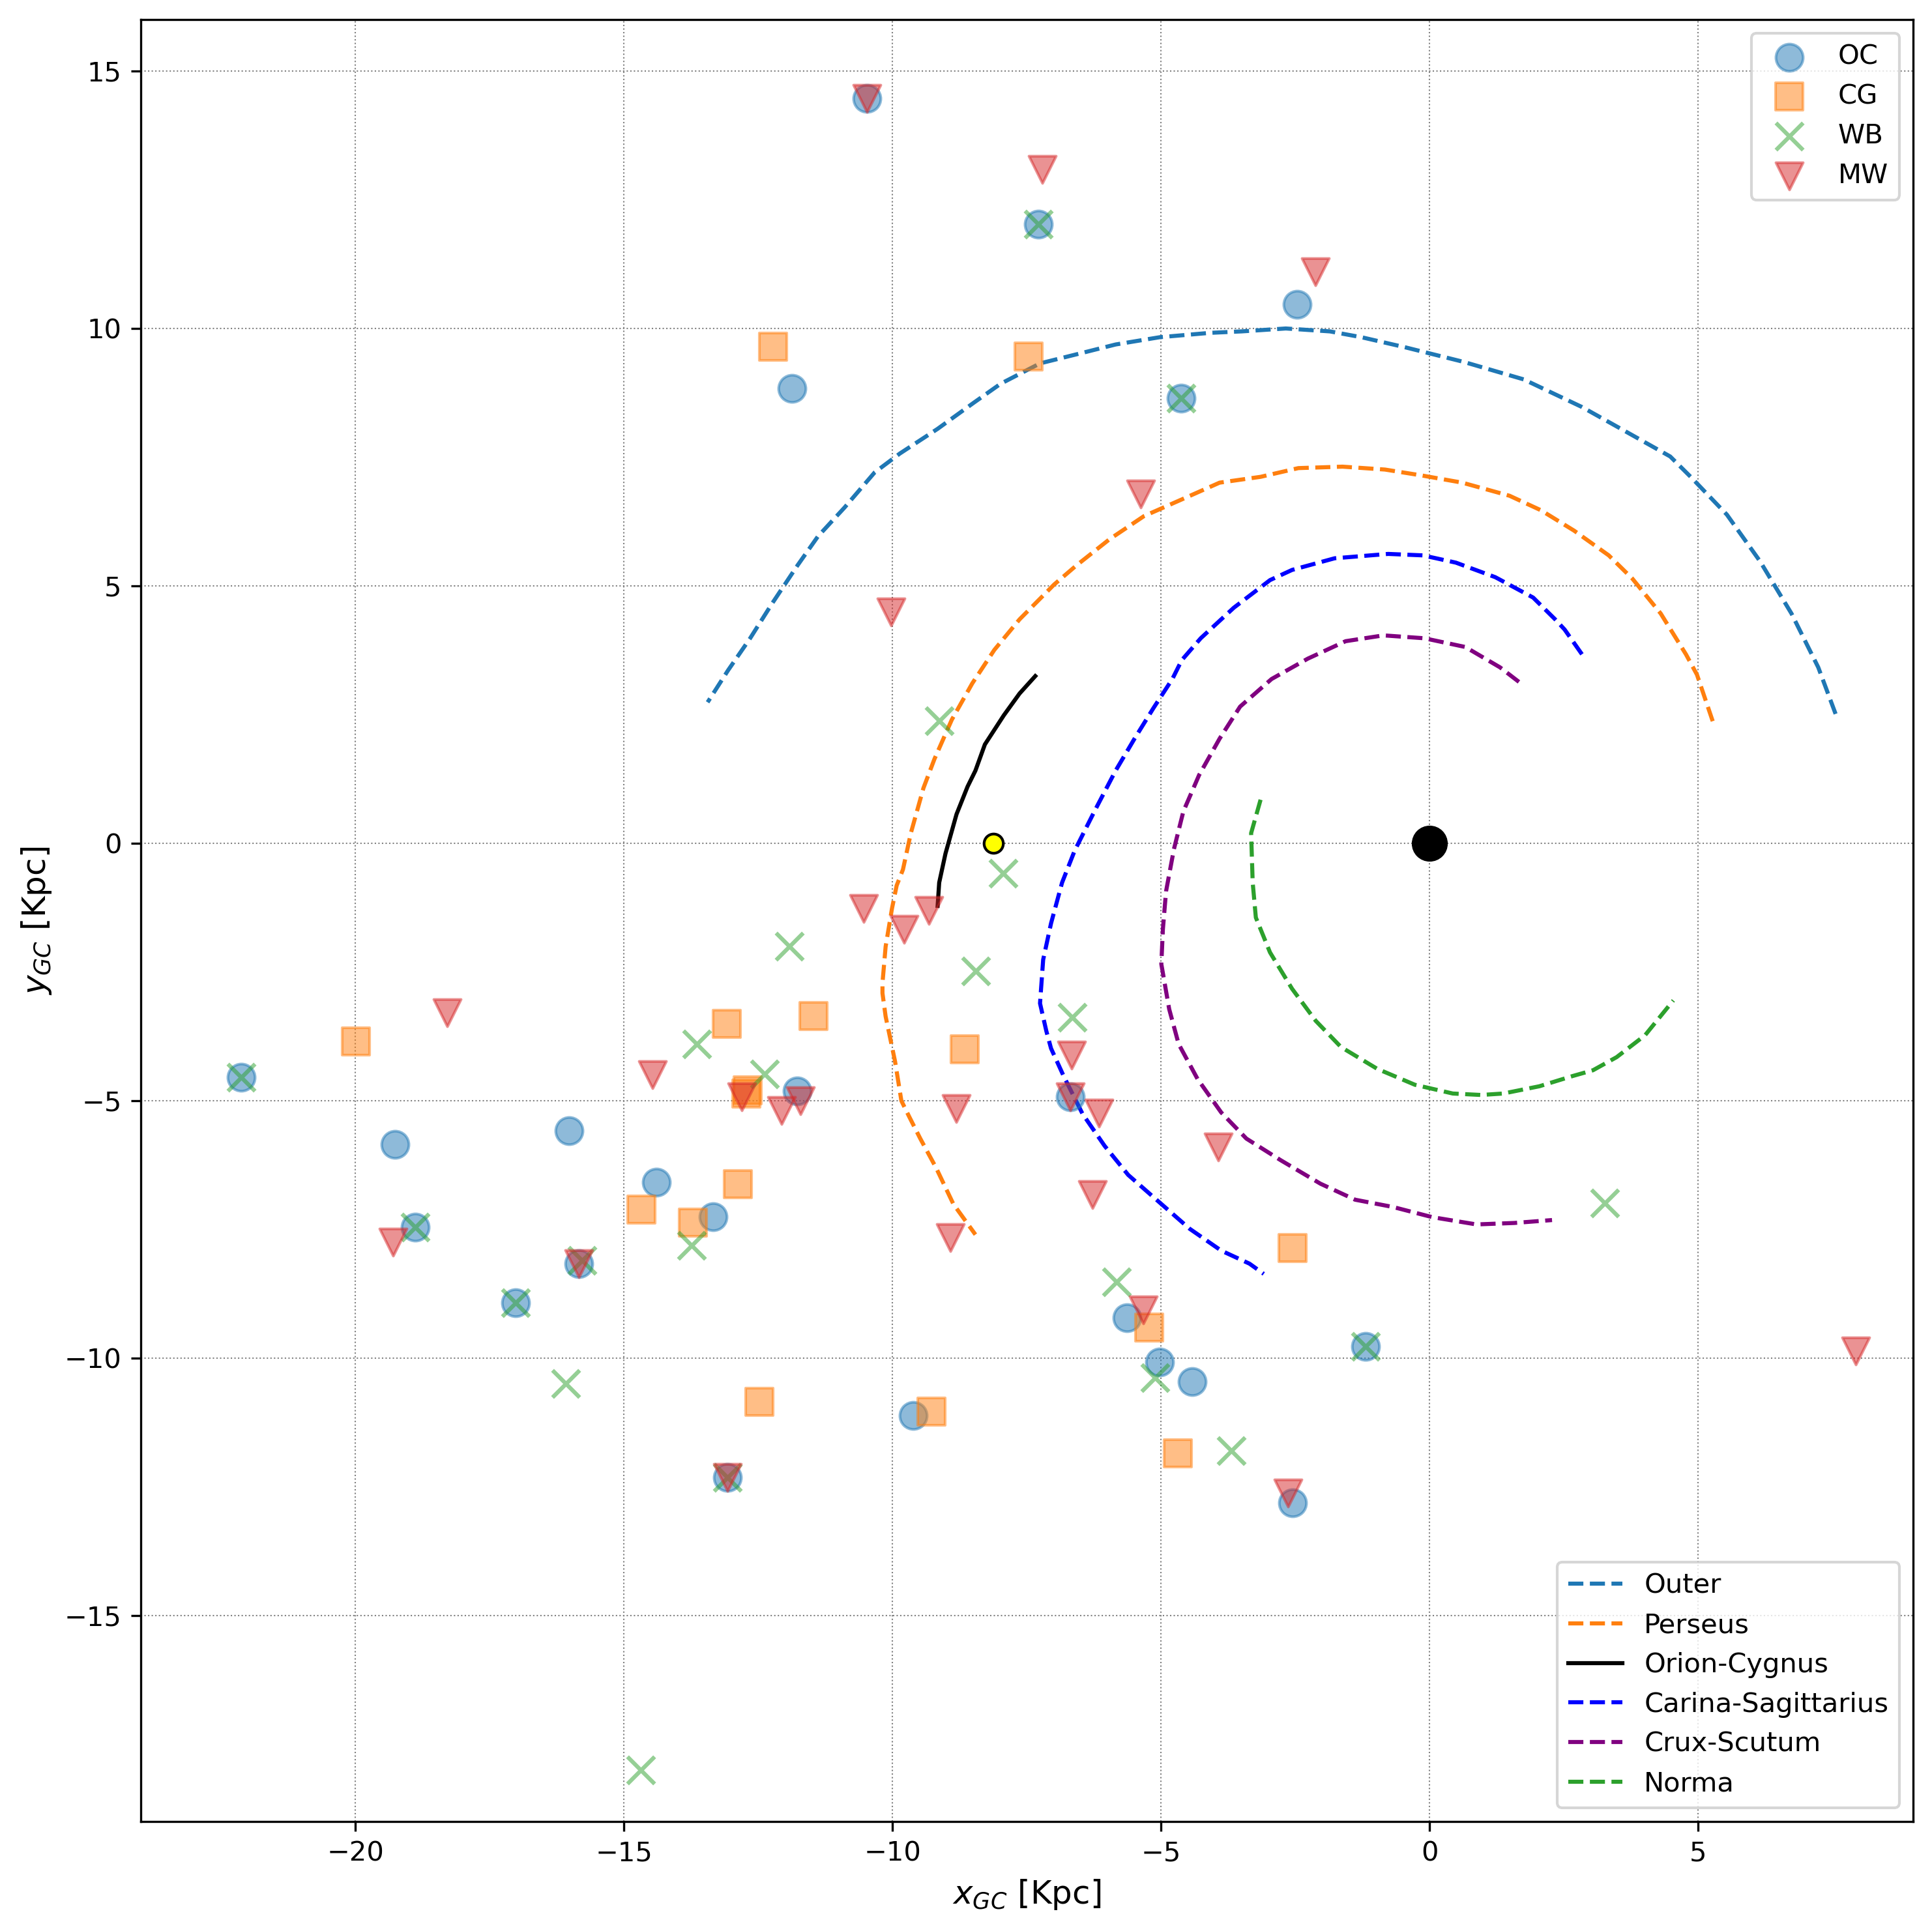
\includegraphics[]{figs/MWmap.png}}
  \caption{xxx}
  \label{fig:MWmap}
 \end{figure*}





% =============================================================================
\section{Cluster analysis}
 \label{sec:clust_analy}

 xxxxx





% =============================================================================
\section{Results}
 \label{sec:results}

 xxxxx





% =============================================================================
\section{Conclusions}
 \label{sec:conclusions}

 xxxxx




   %-------------------------------------- Two column figure (place early!)
   % \begin{figure*}
   % \centering
   % %%%\includegraphics{empty.eps}
   % %%%\includegraphics{empty.eps}
   % %%%\includegraphics{empty.eps}
   % \caption{Adiabatic exponent $\Gamma_1$.
   %             $\Gamma_1$ is plotted as a function of
   %             $\lg$ internal energy $\mathrm{[erg\,g^{-1}]}$ and $\lg$
   %             density $\mathrm{[g\,cm^{-3}]}$.}
   %            \label{FigGam}%
   %  \end{figure*}


   %--------------------------------------------------- One column table
%    \begin{table}
%       \caption[]{Opacity sources.}
%          \label{KapSou}
%      $$ 
%          \begin{array}{p{0.5\linewidth}l}
%             \hline
%             \noalign{\smallskip}
%             Source      &  T / {[\mathrm{K}]} \\
%             \noalign{\smallskip}
%             \hline
%             \noalign{\smallskip}
%             Yorke 1979, Yorke 1980a & \leq 1700^{\mathrm{a}}     \\
% %           Yorke 1979, Yorke 1980a & \leq 1700             \\
%             Kr\"ugel 1971           & 1700 \leq T \leq 5000 \\
%             Cox \& Stewart 1969     & 5000 \leq             \\
%             \noalign{\smallskip}
%             \hline
%          \end{array}
%      $$ 
%    \end{table}



%                                                One column figure
%----------------------------------------------------------------- 
% \begin{figure}
% \centering
% %%%\includegraphics[width=3cm]{empty.eps}
%    \caption{Vibrational stability equation of state
%             $S_{\mathrm{vib}}(\lg e, \lg \rho)$.
%             $>0$ means vibrational stability.
%            }
%       \label{FigVibStab}
% \end{figure}

\section{Conclusions}

xxx

\begin{acknowledgements}
This research has made use of the WEBDA database, operated at the Department of
Theoretical Physics and Astrophysics of the Masaryk University.
%
This research has made use of the VizieR catalog access tool, operated at CDS,
Strasbourg, France~\citep{Ochsenbein_2000}.
%
This research has made use of ``Aladin sky atlas'' developed at
CDS, Strasbourg Observatory, France~\citep{Bonnarel2000,Boch2014}.
%
This research has made use of NASA's Astrophysics Data System.
%
This research made use of the Python language v3.7.3~\citep{vanRossum_1995}
and the following packages:
NumPy\footnote{\url{http://www.numpy.org/}}~\citep{vanDerWalt_2011};
SciPy\footnote{\url{http://www.scipy.org/}}~\citep{Jones_2001};
Astropy\footnote{\url{http://www.astropy.org/}}, a community-developed core
Python package for Astronomy \citep{Astropy_2013};
matplotlib\footnote{\url{http://matplotlib.org/}}~\citep{hunter_2007}
\end{acknowledgements}




\bibliographystyle{aa}
\bibliography{biblio} % your references Yourfile.bib

\end{document}


